\documentclass[12pt, a4paper]{article}
\usepackage[brazilian]{babel} %Traduz o documento para o português brasileiro.
\usepackage[utf8]{inputenc} %Reconhece à acentuação
\usepackage{lipsum} %Gera texto aleatório
\usepackage{graphicx}
\usepackage{subfig}
\usepackage{wrapfig}
\usepackage[leftcaption]{sidecap}

\graphicspath{{imagens/}}

%preâmbulo
\title{Esse é o título do 1º artigo da aula 3}
\author{César Antônio de Magalhães}
\date{\today}

%conteúdo
\begin{document}
	\listoffigures
	
	\section{Exemplos}
		\lipsum[1]
	
		\begin{figure}[htbp]
			\centering
			
\includegraphics[width=0.5\textwidth, height=2cm, angle=45]{img1.jpg}
			\caption{Figura no formato jpeg	}
		\end{figure}
	
		\lipsum[2]
		
		\begin{figure}[htbp]
			\centering
			
\includegraphics[clip, trim= 0 30 0 50]{img2.png}
			\caption{Figura no formato png	}
		\end{figure}
		
		\lipsum[3]
		
		\begin{figure}[hbtp]
			\centering
			
\includegraphics[scale=0.4]{img_angry_birds.jpg}
			\caption{Angry birds}
		\end{figure}
		
		\lipsum[4]
		
		\begin{figure}[hbtp]
			\centering
			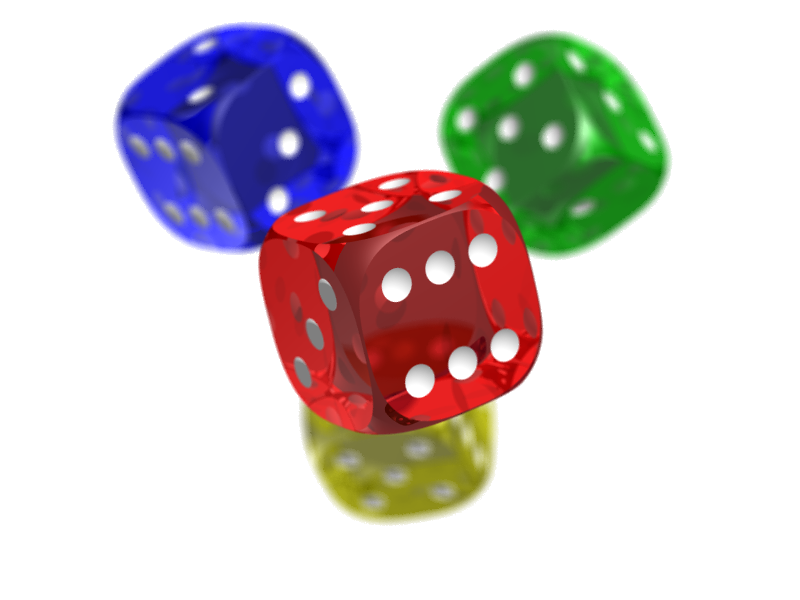
\includegraphics[width=0.5\paperwidth]{img_dados.png}
			\caption{Dados coloridos}
		\end{figure}
		
		\lipsum[5]
		
		\begin{figure}[h]
			\centering
			\subfloat[Primeira figura]{
				
\includegraphics[width=0.2\paperwidth]{img1.jpg}
			}
			\quad\quad
			\subfloat[Segunda figura]{
				
\includegraphics[width=0.2\paperwidth]{img2.png}
			}
			\caption{Duas figuras }
		\end{figure}
		
		\lipsum[6]
		
		\lipsum[7]
		
		\begin{wrapfigure}{l}{0.25\textwidth}
			\centering
			
\includegraphics[width=0.25\textwidth]{img1.jpg}
			\caption{Figura ao lado do texto}
		\end{wrapfigure}
		
				
		\lipsum[8]
		\lipsum[9]
		
		\begin{SCfigure}
			
\includegraphics[width=0.25\textwidth]{img2.png}
			\caption{Figura com legenda ao lado }
		\end{SCfigure}
		
		\lipsum[10]
		
\end{document}
